\documentclass[a4paper]{article}
%%%%%Paquetes%%%%%
\usepackage[T1]{fontenc}
\usepackage[utf8]{inputenc}
\usepackage[spanish]{babel}
\usepackage{amsmath,amssymb,eucal,mathrsfs}
\usepackage[svgnames,x11names]{xcolor}
\usepackage{colortbl}
\usepackage{Estilos/MiEstilo}
%\usepackage{Estilos/Informe}
\usepackage{amsmath}
\usepackage{times}
\usepackage{color}
\usepackage{listings}
\usepackage{graphicx}
\usepackage{caption}

	\setcounter{tocdepth}{2} %Mostrar solo 3 niveles en el índice
		\makeindex	%índice de palabras
		\title{Modelos de Computación.\\ Práctica 4. }
		\author{Luis José Quintana Bolaño}
		\date{\today}

\begin{document}
		\maketitle
		\begin{abstract}
		    Prácticas con el simulador URM.
  		\end{abstract}
		\section{Ejercicio 1}
		Computaciones para el programa
		\begin{verbatim}
		J(2,3,0)
		S(1)
		S(3)
		J(1,1,1)
		\end{verbatim}
  		\subsection{Computación para la entrada $R1=0, R2=0$}
		\begin{equation*}\begin{gathered}
		(1, <R1=0, R2=0, R3=0>) \sim (0, <R1=0, R2=0, R3=0>)
		\end{gathered}\end{equation*}
		\subsection{Computación para la entrada $R1=1, R2=1$}
		\begin{equation*}\begin{gathered}
		(1, <R1=1, R2=1, R3=0>) \sim (2, <R1=1, R2=1, R3=0>) \sim (3, <R1=2, R2=1, R3=0>) \sim\\
		(4, <R1=2, R2=1, R3=1>) \sim (1, <R1=2, R2=1, R3=1>) \sim (0, <R1=2, R2=1, R3=1>)
		\end{gathered}\end{equation*}
		\subsection{Computación para la entrada $R1=1, R2=2$}
		\begin{equation*}\begin{gathered}
		(1, <R1=1, R2=2, R3=0>) \sim (2, <R1=1, R2=2, R3=0>) \sim (3, <R1=2, R2=2, R3=0>) \sim\\
		(4, <R1=2, R2=2, R3=1>) \sim (1, <R1=2, R2=2, R3=1>) \sim (2, <R1=2, R2=2, R3=1>) \sim\\
		(3, <R1=3, R2=2, R3=1>) \sim (4, <R1=3, R2=2, R3=2>) \sim (1, <R1=3, R2=2, R3=2>) \sim\\
		(0, <R1=3, R2=2, R3=2>)
		\end{gathered}\end{equation*}
		\subsection{Computación para la entrada $R1=2, R2=1$}
		\begin{equation*}\begin{gathered}
		(1, <R1=2, R2=1, R3=0>) \sim (2, <R1=2, R2=1, R3=0>) \sim (3, <R1=3, R2=1, R3=0>) \sim\\
		(4, <R1=3, R2=1, R3=1>) \sim (1, <R1=3, R2=1, R3=1>) \sim (0, <R1=3, R2=1, R3=1>)
		\end{gathered}\end{equation*}

		\section{Ejercicio 2}
		El programa
		\begin{verbatim}
		J(1,2,3)
		J(1,1,4)
		S(2)
		T(2,1)
		\end{verbatim}
		calcula la función
		\begin{equation*}
  			f(x) = \left\{ 
  			\begin{array}{rl}
  				x & \text{si } x>0 \\
  				1 & \text{en otro caso} 
  			\end{array} \right.
  		\end{equation*}

		\section{Ejercicio 3}
  		Código propuesto para el programa "bloque de transferencia":
  		\begin{verbatim}
  		T(1,2)
  		J(1,1,1)
  		\end{verbatim}

  		\section{Ejercicio 4}
  		Computaciones para el programa
  		\begin{verbatim}
		J(1,4,10)
		T(1,4)
		S(2)
		J(1,2,10)
		Z(3)
		S(3)
		S(4)
		J(1,3,3)
		J(1,1,6)
		T(4,1)
  		\end{verbatim}
  		\subsection{Computación para la entrada $R1=0$}
  		\begin{equation*}\begin{gathered}
		(1, <R1=0, R2=0, R3=0, R4=0>) \sim (10, <R1=0, R2=0, R3=0, R4=0>) \sim\\
		(11, <R1=0, R2=0, R3=0, R4=0>)
		\end{gathered}\end{equation*}
		\begin{figure}[H]
  			\centering
  			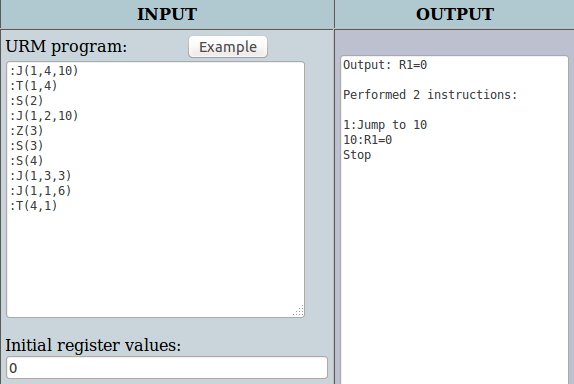
\includegraphics[scale=0.5]{images/40.png}
  		\end{figure}
		\subsection{Computación para la entrada $R1=1$}
  		\begin{equation*}\begin{gathered}
		(1, <R1=1, R2=0, R3=0, R4=0>) \sim (2, <R1=1, R2=0, R3=0, R4=0>) \sim\\
		(3, <R1=1, R2=0, R3=0, R4=1>) \sim (4, <R1=1, R2=1, R3=0, R4=1>) \sim\\
		(10, <R1=1, R2=1, R3=0, R4=1>) \sim (11, <R1=1, R2=1, R3=0, R4=1>)
		\end{gathered}\end{equation*}
		\begin{figure}[H]
  			\centering
  			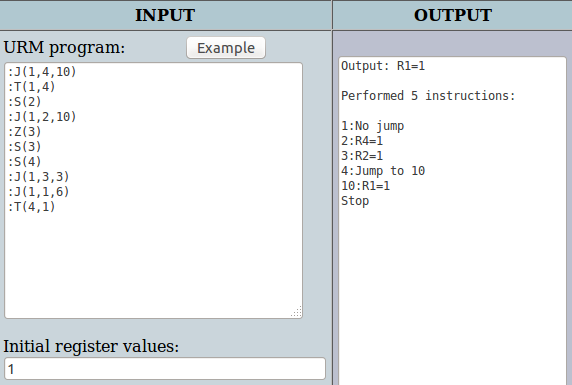
\includegraphics[scale=0.5]{images/41.png}
  		\end{figure}
		\subsection{Computación para la entrada $R1=2$}
		\begin{equation*}\begin{gathered}
		(1, <R1=2, R2=0, R3=0, R4=0>) \sim (2, <R1=2, R2=0, R3=0, R4=0>) \sim\\
		(3, <R1=2, R2=0, R3=0, R4=2>) \sim (4, <R1=2, R2=1, R3=0, R4=2>) \sim\\
		(5, <R1=2, R2=1, R3=0, R4=2>) \sim (6, <R1=2, R2=1, R3=0, R4=2>) \sim\\
		(7, <R1=2, R2=1, R3=1, R4=2>) \sim (8, <R1=2, R2=1, R3=1, R4=3>) \sim\\ 
		(9, <R1=2, R2=1, R3=1, R4=3>) \sim (6, <R1=2, R2=1, R3=1, R4=3>) \sim\\
		(7, <R1=2, R2=1, R3=2, R4=3>) \sim (8, <R1=2, R2=1, R3=2, R4=4>) \sim\\
		(3, <R1=2, R2=1, R3=2, R4=4>) \sim (4, <R1=2, R2=2, R3=2, R4=4>) \sim\\
		(10, <R1=2, R2=2, R3=2, R4=4>) \sim (11, <R1=4, R2=2, R3=2, R4=4>)
		\end{gathered}\end{equation*}
		\begin{figure}[H]
  			\centering
  			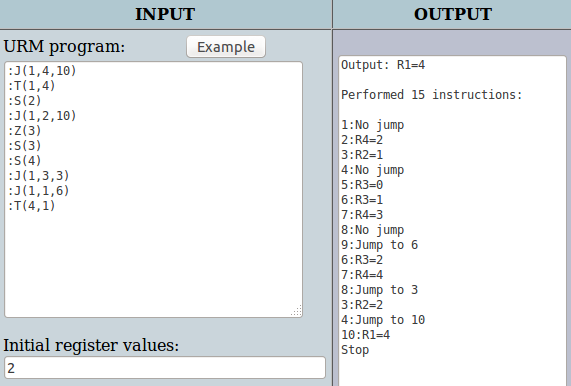
\includegraphics[scale=0.5]{images/42.png}
  		\end{figure}
		\subsection{Computación para la entrada $R1=3$}
		\begin{equation*}\begin{gathered}
		(1, <R1=3, R2=0, R3=0, R4=0>) \sim (2, <R1=3, R2=0, R3=0, R4=0>) \sim\\
		(3, <R1=3, R2=0, R3=0, R4=3>) \sim (4, <R1=3, R2=1, R3=0, R4=3>) \sim\\
		(5, <R1=3, R2=1, R3=0, R4=3>) \sim (6, <R1=3, R2=1, R3=0, R4=3>) \sim\\
		(7, <R1=3, R2=1, R3=1, R4=3>) \sim (8, <R1=3, R2=1, R3=1, R4=4>) \sim\\
		(9, <R1=3, R2=1, R3=1, R4=4>) \sim (6, <R1=3, R2=1, R3=1, R4=4>) \sim\\
		(7, <R1=3, R2=1, R3=2, R4=4>) \sim (8, <R1=3, R2=1, R3=2, R4=5>) \sim\\
		(9, <R1=3, R2=1, R3=2, R4=5>) \sim (6, <R1=3, R2=1, R3=2, R4=5>) \sim\\
		(7, <R1=3, R2=1, R3=3, R4=5>) \sim (8, <R1=3, R2=1, R3=3, R4=6>) \sim\\
		(3, <R1=3, R2=1, R3=3, R4=6>) \sim (4, <R1=3, R2=2, R3=3, R4=6>) \sim\\
		(5, <R1=3, R2=2, R3=3, R4=6>) \sim (6, <R1=3, R2=2, R3=0, R4=6>) \sim\\
		(7, <R1=3, R2=2, R3=1, R4=6>) \sim (8, <R1=3, R2=2, R3=1, R4=7>) \sim\\
		(9, <R1=3, R2=2, R3=1, R4=7>) \sim (6, <R1=3, R2=2, R3=1, R4=7>) \sim\\
		(7, <R1=3, R2=2, R3=2, R4=7>) \sim (8, <R1=3, R2=2, R3=2, R4=8>) \sim\\
		(9, <R1=3, R2=2, R3=2, R4=8>) \sim (6, <R1=3, R2=2, R3=2, R4=8>) \sim\\
		(7, <R1=3, R2=2, R3=3, R4=8>) \sim (8, <R1=3, R2=2, R3=3, R4=9>) \sim\\
		(3, <R1=3, R2=2, R3=3, R4=9>) \sim (4, <R1=3, R2=3, R3=3, R4=9>) \sim\\
		(10, <R1=3, R2=3, R3=3, R4=9>) \sim (11, <R1=9, R2=3, R3=3, R4=9>)
		\end{gathered}\end{equation*}
		\begin{figure}[H]
  			\centering
  			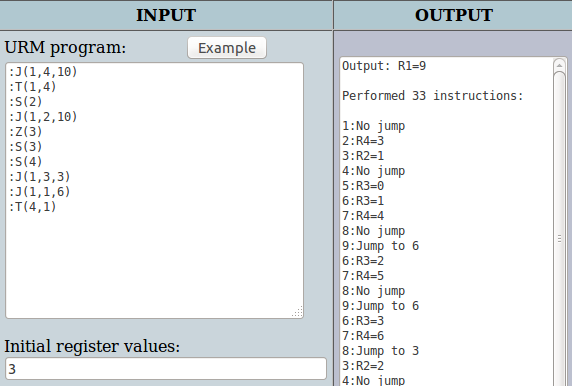
\includegraphics[scale=0.5]{images/43.png}
  		\end{figure}
		\subsection{Función calculada}
		El programa calcula la función
		\begin{equation*}
  			f(x) = x*x
  		\end{equation*}

  		\section{Ejercicio 5}
  		Computaciones para el programa
  		\begin{verbatim}
		J(2,3,5)
		S(1)
		S(3)
		J(1,1,1)
  		\end{verbatim}
  		\subsection{Computación para la entrada $R1=0$, $R2=0$}
  		\begin{equation*}\begin{gathered}
		(1, <R1=0, R2=0, R3=0>) \sim (5, <R1=0, R2=0, R3=0>)
		\end{gathered}\end{equation*}
		\begin{figure}[H]
  			\centering
  			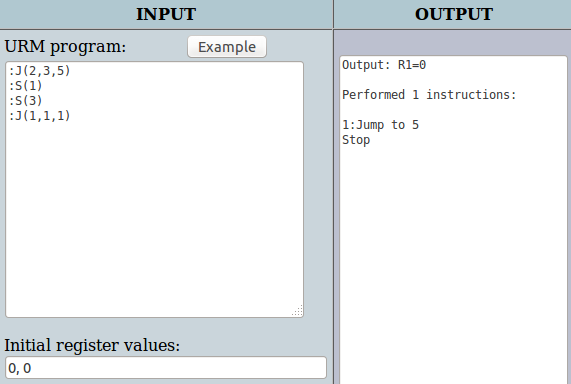
\includegraphics[scale=0.5]{images/500.png}
  		\end{figure}
		\subsection{Computación para la entrada $R1=1$, $R2=0$}
		\begin{equation*}\begin{gathered}
		(1, <R1=1, R2=0, R3=0>) \sim (5, <R1=1, R2=0, R3=0>)
		\end{gathered}\end{equation*}
		\begin{figure}[H]
  			\centering
  			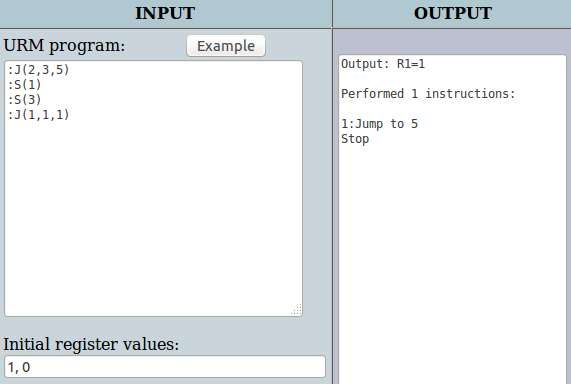
\includegraphics[scale=0.5]{images/510.png}
  		\end{figure}
		\subsection{Computación para la entrada $R1=0$, $R2=1$}
		\begin{equation*}\begin{gathered}
		(1, <R1=0, R2=1, R3=0>) \sim (2, <R1=0, R2=1, R3=0>) \sim (3, <R1=1, R2=1, R3=0>) \sim\\
		(4, <R1=1, R2=1, R3=1>) \sim (1, <R1=1, R2=1, R3=1>) \sim (5, <R1=1, R2=1, R3=1>)
		\end{gathered}\end{equation*}
		\begin{figure}[H]
  			\centering
  			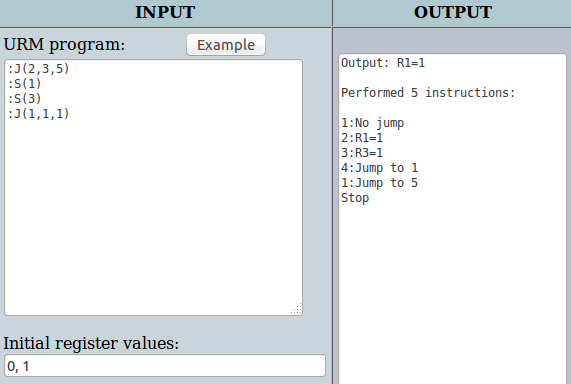
\includegraphics[scale=0.5]{images/501.png}
  		\end{figure}
		\subsection{Computación para la entrada $R1=1$, $R2=1$}
		\begin{equation*}\begin{gathered}
		(1, <R1=1, R2=1, R3=0>) \sim (2, <R1=1, R2=1, R3=0>) \sim (3, <R1=2, R2=1, R3=0>) \sim\\
		(4, <R1=2, R2=1, R3=1>) \sim (1, <R1=2, R2=1, R3=1>) \sim (5, <R1=2, R2=1, R3=1>)
		\end{gathered}\end{equation*}
		\begin{figure}[H]
  			\centering
  			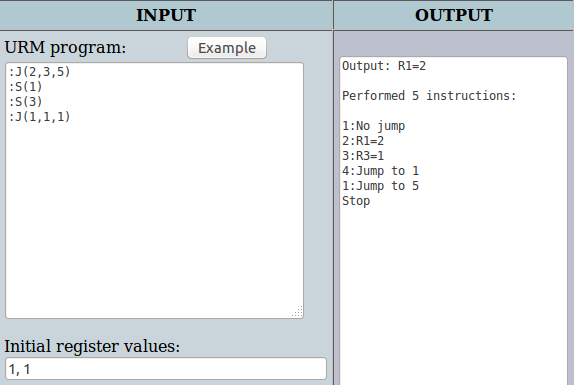
\includegraphics[scale=0.5]{images/511.png}
  		\end{figure}
		\subsection{Función calculada}
		El programa calcula la función
		\begin{equation*}
  			f(x_1, x_2) = x_1+x_2
  		\end{equation*}

  		\section{Ejercicio 6}
	Computaciones para el programa
	\begin{verbatim}
	J(1,2,6)
	S(3)
	S(2)
	J(1,1,1)
	Z(0)
	J(1,3,10)
	S(1)
	J(1,1,7)
	\end{verbatim}
	\subsection{Computación para la entrada $R1=0$}
	\begin{equation*}\begin{gathered}
	(1, <R1=0, R2=0, R3=0>) \sim (6, <R1=0, R2=0, R3=0>) \sim (9, <R1=0, R2=0, R3=0>)
	\end{gathered}\end{equation*}
	\begin{figure}[H]
  		\centering
  		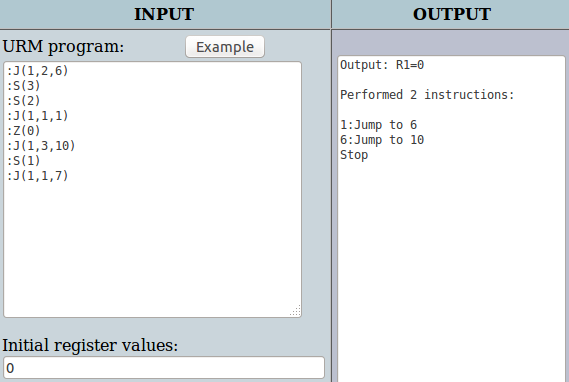
\includegraphics[scale=0.5]{images/60.png}
  	\end{figure}
	\subsection{Computación para la entrada $R1=1$}
	\begin{equation*}\begin{gathered}
	(1, <R1=1, R2=0, R3=0>) \sim (2, <R1=1, R2=0, R3=0>) \sim (3, <R1=1, R2=0, R3=1>) \sim\\
	(4, <R1=1, R2=1, R3=1>) \sim (1, <R1=1, R2=1, R3=1>) \sim (6, <R1=1, R2=1, R3=1>) \sim\\
	(9, <R1=1, R2=1, R3=1>)
	\end{gathered}\end{equation*}
	\begin{figure}[H]
  		\centering
  		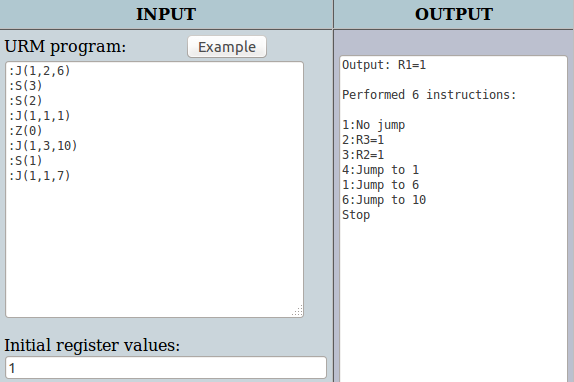
\includegraphics[scale=0.5]{images/61.png}
  	\end{figure}
	\subsection{COmputación para la entrada $R1=2$}
	\begin{equation*}\begin{gathered}
	(1, <R1=2, R2=0, R3=0>) \sim (2, <R1=2, R2=0, R3=0>) \sim (3, <R1=2, R2=0, R3=1>) \sim\\
	(4, <R1=2, R2=1, R3=1>) \sim (1, <R1=2, R2=1, R3=1>) \sim (2, <R1=2, R2=1, R3=1>) \sim\\
	(3, <R1=2, R2=1, R3=2>) \sim (4, <R1=2, R2=2, R3=2>) \sim (1, <R1=2, R2=2, R3=2>) \sim\\
	(6, <R1=2, R2=2, R3=2>) \sim (9, <R1=2, R2=2, R3=2>)
	\end{gathered}\end{equation*}
	\begin{figure}[H]
  		\centering
  		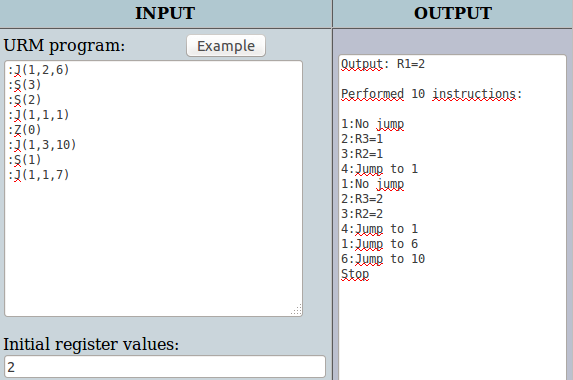
\includegraphics[scale=0.5]{images/62.png}
  	\end{figure}
	\subsection{Compuación para la entrada $R1=3$}
	\begin{equation*}\begin{gathered}
	(1, <R1=3, R2=0, R3=0>) \sim (2, <R1=3, R2=0, R3=0>) \sim (3, <R1=3, R2=0, R3=1>) \sim\\
	(4, <R1=3, R2=1, R3=1>) \sim (1, <R1=3, R2=1, R3=1>) \sim (2, <R1=3, R2=1, R3=1>) \sim\\
	(3, <R1=3, R2=1, R3=2>) \sim (4, <R1=3, R2=2, R3=2>) \sim (1, <R1=3, R2=2, R3=2>) \sim\\
	(2, <R1=3, R2=2, R3=2>) \sim (3, <R1=3, R2=2, R3=3>) \sim (4, <R1=3, R2=3, R3=3>) \sim\\
	(1, <R1=3, R2=3, R3=3>)(6, <R1=3, R2=3, R3=3>) \sim (9, <R1=3, R2=3, R3=3>)
	\end{gathered}\end{equation*}
	\begin{figure}[H]
  		\centering
  		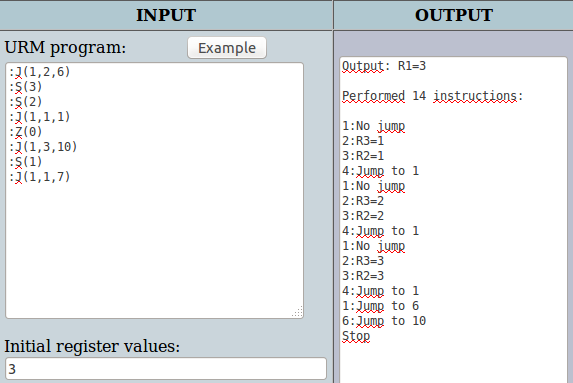
\includegraphics[scale=0.5]{images/63.png}
  	\end{figure}
	\subsection{Función calculada}
	El programa calcula la función
	\begin{equation*}
		f(x)=x
	\end{equation*}

  		\section{Ejercicio 7}
	Computaciones para el programa
	\begin{verbatim}
	J(2,3,9)
	J(1,3,9)
	S(3)
	S(4)
	J(2,4,7)
	J(1,1,2)
	Z(4)
	J(1,1,2)
	T(4,1)
	\end{verbatim}
	\subsection{Computación para la entrada $R1=0$, $R2=0$}
	\begin{equation*}\begin{gathered}
	(1, <R1=0, R2=0, R3=0, R4=0>) \sim (9, <R1=0, R2=0, R3=0, R4=0>) \sim\\
	(10, <R1=0, R2=0, R3=0, R4=0>)
	\end{gathered}\end{equation*}
	\subsection{Computación para la entrada $R1=0$, $R2=1$}
	\begin{equation*}\begin{gathered}
	(1, <R1=0, R2=1, R3=0, R4=0>) \sim (2, <R1=0, R2=1, R3=0, R4=0>) \sim\\
	(9, <R1=0, R2=1, R3=0, R4=0>) \sim (10, <R1=0, R2=1, R3=0, R4=0>)
	\end{gathered}\end{equation*}
	\subsection{Computación para la entrada $R1=1$, $R2=0$}
	\begin{equation*}\begin{gathered}
	(1, <R1=1, R2=0, R3=0, R4=0>) \sim (9, <R1=1, R2=0, R3=0, R4=0>) \sim\\
	(10, <R1=0, R2=0, R3=0, R4=0>)
	\end{gathered}\end{equation*}
	\subsection{Computación para la entrada $R1=1$, $R2=1$}
	\begin{equation*}\begin{gathered}
	(1, <R1=1, R2=1, R3=0, R4=0>) \sim (2, <R1=1, R2=1, R3=0, R4=0>) \sim\\
	(3, <R1=1, R2=1, R3=0, R4=0>) \sim (4, <R1=1, R2=1, R3=1, R4=0>) \sim\\
	(5, <R1=1, R2=1, R3=1, R4=1>) \sim (7, <R1=1, R2=1, R3=1, R4=1>) \sim\\
	(8, <R1=1, R2=1, R3=1, R4=0>) \sim (2, <R1=1, R2=1, R3=1, R4=0>) \sim\\
	(9, <R1=1, R2=1, R3=1, R4=0>) \sim (10, <R1=0, R2=1, R3=1, R4=0>)
	\end{gathered}\end{equation*}
	\subsection{Función calculada}
	El programa calcula la función
	\begin{equation*}
		f(x_1, x_2)= \left\{ 
  		\begin{array}{rl}
  				x_1 \bmod x_2 & \text{si } x_2>0 \\
  				0 & \text{en otro caso} 
  		\end{array} \right.
	\end{equation*}

  		\section{Ejercicio 8}
	Computaciones para el programa
	\begin{verbatim}
	T(1,3)
	J(2,3,10)
	S(2)
	S(1)
	S(1)
	J(1,1,2)
	\end{verbatim}
	\subsection{Computación para la entrada $R1=0$}
	\begin{equation*}\begin{gathered}
	(1, <R1=0, R2=0, R3=0>) \sim (2, <R1=0, R2=0, R3=0>) \sim (7, <R1=0, R2=0, R3=0>)
	\end{gathered}\end{equation*}
	\begin{figure}[H]
  		\centering
  		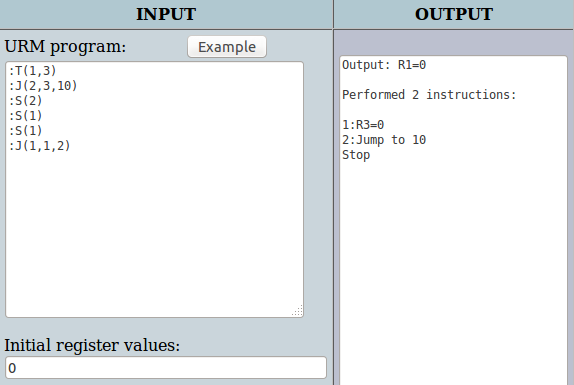
\includegraphics[scale=0.5]{images/80.png}
  	\end{figure}
	\subsection{Computación para la entrada $R1=1$}
	\begin{equation*}\begin{gathered}
	(1, <R1=1, R2=0, R3=0>) \sim (2, <R1=1, R2=0, R3=1>) \sim (3, <R1=1, R2=0, R3=1>) \sim\\
	(4, <R1=1, R2=1, R3=1>) \sim (5, <R1=2, R2=1, R3=1>) \sim (6, <R1=3, R2=1, R3=1>) \sim\\
	(2, <R1=3, R2=1, R3=1>) \sim (7, <R1=3, R2=1, R3=1>)
	\end{gathered}\end{equation*}
	\begin{figure}[H]
  		\centering
  		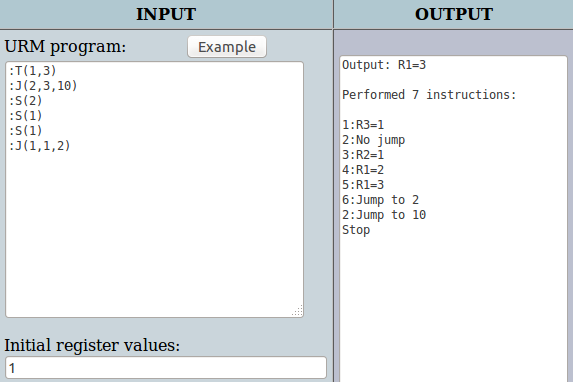
\includegraphics[scale=0.5]{images/81.png}
  	\end{figure}
	\subsection{Computación para la entrada $R1=2$}
	\begin{equation*}\begin{gathered}
	(1, <R1=2, R2=0, R3=0>) \sim (2, <R1=2, R2=0, R3=2>) \sim (3, <R1=2, R2=0, R3=2>) \sim\\
	(4, <R1=2, R2=1, R3=2>) \sim (5, <R1=3, R2=1, R3=2>) \sim (6, <R1=4, R2=1, R3=2>) \sim\\
	(2, <R1=4, R2=1, R3=2>) \sim (3, <R1=4, R2=1, R3=2>) \sim (4, <R1=4, R2=2, R3=2>) \sim\\
	(5, <R1=5, R2=2, R3=2>) \sim (6, <R1=6, R2=2, R3=2>) \sim (2, <R1=6, R2=2, R3=2>) \sim\\
	(7, <R1=6, R2=2, R3=2>)
	\end{gathered}\end{equation*}
	\begin{figure}[H]
  		\centering
  		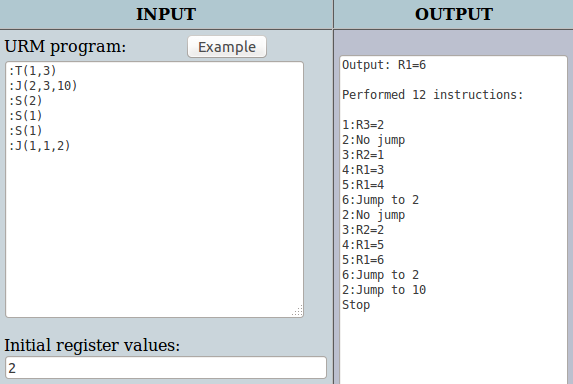
\includegraphics[scale=0.5]{images/82.png}
  	\end{figure}
	\subsection{Computación para la entrada $R1=3$}
	\begin{equation*}\begin{gathered}
	(1, <R1=3, R2=0, R3=0>) \sim (2, <R1=3, R2=0, R3=3>) \sim (3, <R1=3, R2=0, R3=3>) \sim\\
	(4, <R1=3, R2=1, R3=3>) \sim (5, <R1=4, R2=1, R3=3>) \sim (6, <R1=5, R2=1, R3=3>) \sim\\
	(2, <R1=5, R2=1, R3=3>) \sim (3, <R1=5, R2=1, R3=3>) \sim (4, <R1=5, R2=2, R3=3>) \sim\\
	(5, <R1=6, R2=2, R3=3>) \sim (6, <R1=7, R2=2, R3=3>) \sim (2, <R1=7, R2=2, R3=3>) \sim\\
	(3, <R1=7, R2=2, R3=3>) \sim (4, <R1=7, R2=3, R3=3>) \sim (5, <R1=8, R2=3, R3=3>) \sim\\
	(6, <R1=9, R2=3, R3=3>) \sim (2, <R1=9, R2=3, R3=3>) \sim (7, <R1=9, R2=3, R3=3>)
	\end{gathered}\end{equation*}
	\begin{figure}[H]
  		\centering
  		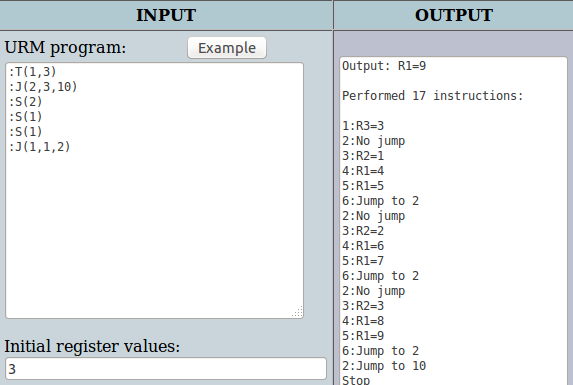
\includegraphics[scale=0.5]{images/83.png}
  	\end{figure}
	\subsection{Función calculada}
	El programa calcula la función
	\begin{equation*}
		f(x)=3x
	\end{equation*}

\end{document}
